\lettrine{C}{entral to this study} is the mechanism by which China may influence the countries it has linkages with. Diffusion theory teach us that there are many ways in which international factors can affect the level of, first and foremost, democracy, but also the level of freedom of expression a populace enjoys. To truly understand how the independent variable links to the dependent variable, a more detailed treatment of this relationship is necessary.

To remind the reader, the research question asks whether a country's linkages to China affect the extent of freedom of expression in that country. It is not immediately obvious that the linkages should have this effect, but in this chapter, I propose first that they do, and second that the effect of linkages will be moderated by regime type. I believe there to be three main reasons for why linkages can impact freedom of expression. These are: learning, immunity, and displacement. Where learning refers to linkages enabling countries to learn from China. Immunity refers to being supported by China when in the process of autocratisation. And lastly, displacement refers to how China is displacing Western democratic countries as a favoured partner, thereby weakening the democratic influence capacity Western countries have on their partner countries.

\section{The Framework}
In this section I construct the framework for studying how dyadic linkages might influence freedom of expression. This framework is built up around the three mechanisms mentioned briefly above and will be expanded on in due time. Here I show the rough outline of my theory, before further elaborating on each mechanism in the next three sections. 

I have noted the importance of the mechanisms proposed by \citet{tansey_ties_2017} and I use this as a base for my theoretical framework. However, I have made a few alterations to based on new evidence \citep{weyland_autocratic_2017}. First of all, I expect \textit{domestic stakeholders} to push for restrict of freedom of expression. As China is not a missionary country, I consider the impetus to restrict freedom of repression to come from the countries themselves. The linkages can only serve to incentivise the domestic actors to restrict freedom of expression. Because I intend to explain the behaviour of the domestic actors, so the domestic stakeholders' willingness to restrict freedom of expression is an assumption not a mechanism in my model. However, I consider it likely that with fewer linkages to China, a domestic stakeholder is more restricted in repressing freedom of expression.

What are the incentives linkages to China give the domestic stakeholders? The mechanisms of \textit{learning} and \textit{decreased salience of autocratic abuse} (see the third and fourth mechanisms in Table \ref{tab:linkage}) are going to continue to play a big part in my own theoretical framework. However, the latter will be named \textit{immunity} for simplicity, as I consider the main purpose of this mechanism to be to achieve immunity from the consequences of restricting freedom of expression.

In contrast, the second mechanism of \citeauthor{tansey_ties_2017} -- \textit{external stakeholders}, which in my case is China -- will not feature in my framework. The reason for this is that some contributions find only limited support for this mechanism in regard to China \citep{chen_democracy_2015}. In its stead I include a mechanism I have chosen to call \textit{displacement}, a term I use for the phenomenon where linkages to China displaces those of Western countries. The reason for including it is that, as China becomes more prominent in the international order, it will start to take more space. This space was previously occupied by Western countries, but with their influence diminishing they have less sway over other countries. I consider it likely that Western democratic countries engage in some form democracy support, showing strong support for freedom of expression \citep{levitsky_linkage_2006}\footnote{Accepting that this is not always what happens \citep{chen_democracy_2015, wong_chinese_2019}}. When their influence is lessened, the pressure to uphold freedom of expression decreases.

\begin{figure}[!hbt]
\centering
\resizebox{.8\textwidth}{!}{%
\begin{circuitikz}
\tikzstyle{every node}=[font=\LARGE]
\draw [ rounded corners = 16.2] (5,16) rectangle  node {\LARGE Linkages to China} (12.5,13.5);
\draw [ rounded corners = 16.2] (6.25,12.25) rectangle  node {\LARGE Immunity} (11.25,9.75);
\draw [ rounded corners = 16.2] (0,12.25) rectangle  node {\LARGE Learning} (5,9.75);
\draw [ rounded corners = 16.2] (12.5,12.25) rectangle  node {\LARGE Displacement} (17.5,9.75);
\draw [ rounded corners = 16.2] (3.75,8.5) rectangle  node {\LARGE Decline in freedom of expression} (13.75,6);
\draw [->, >=Stealth] (8.75,13.5) -- (8.75,12.25);
\draw [short] (5,14.75) -- (2.5,14.75);
\draw [->, >=Stealth] (2.5,14.75) -- (2.5,12.25);
\draw [->, >=Stealth] (8.75,9.75) -- (8.75,8.5);
\draw [short] (2.5,9.75) -- (2.5,7.25);
\draw [->, >=Stealth] (2.5,7.25) -- (3.75,7.25);
\draw [->, >=Stealth] (15,14.75) -- (15,12.25);
\draw [ rounded corners = 16.2, dashed] (0,19.75) rectangle  node {\LARGE Patron-seeking}  (7.5,17.25);
\draw [ rounded corners = 16.2, dashed] (10,19.75) rectangle  node {\LARGE Economic necessity}  (17.5,17.25);
\draw [->, >=Stealth, dashed] (6.25,17.25) -- (6.25,16);
\draw [->, >=Stealth, dashed] (11.25,17.25) -- (11.25,16);

\draw [short] (12.5,14.75) -- (15,14.75);
\draw [short] (15,9.75) -- (15,7.25);
\draw [->, >=Stealth] (15,7.25) -- (13.75,7.25);
\end{circuitikz}
}%
\caption{Theory of Chinese influence}
\label{fig:theory}
\end{figure}

My theory can be summed up by Figure \ref{fig:theory}. First, I take for granted that most countries wish to establish closer linkages to China. In some cases, this might happen because some regimes try to create a good rapport with an autocratic patron, or, and what is more likely, it happens because it is all but an economic necessity to establish closer linkages to China. This is reflected in Figure \ref{fig:link-china}, that shows how linkages to China have developed in the years between 1994 and 2023. The assumptions of why countries chose to establish linkages to China is represented by the two dashed boxes in the upper part of Figure \ref{fig:theory}. However, an in-depth enquiry into the reason for the establishment of linkages is beyond the scope of this study. It should suffice it to say that China is today by far the most powerful autocracy in the world as its economic power is second only to the USA \citep{imf_world_2025}. 

\begin{figure}
    \centering
    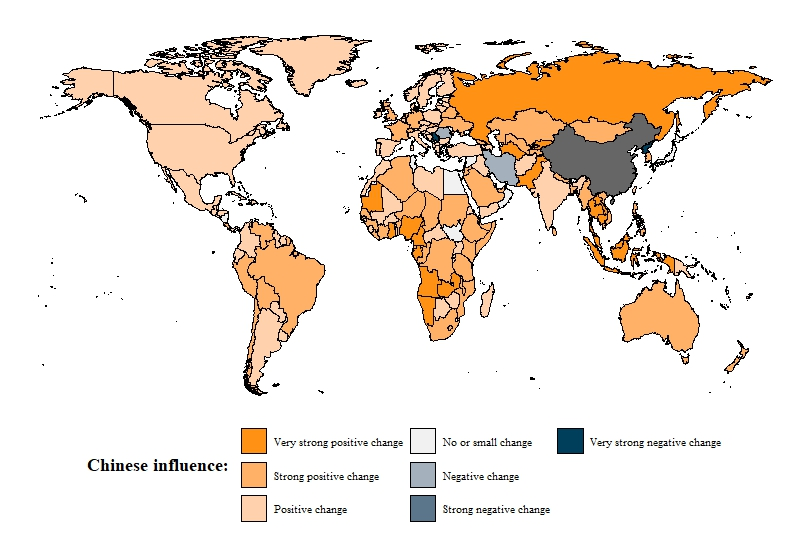
\includegraphics[width=\linewidth]{graphics/chinese_influence.jpeg}
    \caption{Development of linkages to China 1994-2023}
    \label{fig:link-china}
\end{figure}

When linkages are established, the influence of China can start to have an effect on freedom of expression. Whether it is a supply or demand relationship is unclear. Authors have attributed it to both \citep[e.g., see:][]{ambrosio_rise_2012, bader_china_2015, brand_authoritarian_2015, economy_exporting_2020, gamso_is_2021, loughlin_chinese_2021, risse_democracy_2015, toettoe_foreign_2023, weyland_autocratic_2017}; however, the literature indicates the latter to be more plausible, with the caveat that China is using the opportunity for what it is worth. I therefore consider linkages, if they have an effect at all, to be a demand-driven mechanism, see Table \ref{tab:mechanism} for more information on this point. 

The next level of Figure \ref{fig:theory} are the three mechanisms: learning, immunity, and displacement. Since this are the main parts of my theory, the next sections explain these three mechanisms in greater detail and how they might cause a decline in freedom of expression.

\section{Learning}
Learning is in several contributions theorised to be one of the main vehicles of policy diffusion \citep{gilardi_four_2016, shipan_mechanisms_2008, simmons_introduction_2006}; this is not surprising as actors want to strengthen their position by using whatever methods seems to them most effective. And to do this, they look to their peers for guidance. I focus here on learning, as I see decision makers as generally being rational in adopting policies which are either for personal gain or as an end in themselves, i.e., to strengthen their country \citep{shipan_mechanisms_2008}, and believe that it is one of the main vehicles for linkages to China to have an impact on freedom of expression.

What I have simplified in this thesis as the category of `learning', is in the literature quite often divided into two separate mechanisms: learning and imitation/emulation \citep{ elkins_waves_2005, gilardi_four_2016, shipan_mechanisms_2008}. There might not seem to be all that much difference between them, and I would argue that in most cases there is not; however, in some cases they might be usefully separated. Learning, when used as a separate category can be defined as adopting policies after studying their effects in other places and deeming them the best option. Imitation on the other hand is defined as the adoption of policies based on their earlier adoption by peers and the appropriateness of the policy to the polity \citep[pp. 799-801]{simmons_introduction_2006}. There is much more that can be said about this difference; but, except in noting the use, it will not be relevant to distinguish between these mechanisms. The reason is that the outcome, introduction of a certain policy is similar. I therefore collapsed learning and immitation into a single category: learning. 

\subsection{Learning and China}

Diplomatic linkages are probably the main way learning can have an effect on the diffusion of policy. \citet[p. 385]{levitsky_linkage_2006} argues that `[l]inkages generates ``soft power,'' or the ability to ``shape preferences'' and ``get others to do what you want.''' Here diplomatic linkages are one way of achieving this, especially for dominant countries like China and Russia, which smaller countries would look to learn from.

Diplomatic linkages show how interconnected two polities are and can include measures like the establishment of embassies and consulates, visits by high-level officials, and participation in international organisations. With repeated interactions in these forums, countries may influence each other as they learn about the policies that the partners have enacted. 

This effect can occur through socialisation, conditionality, and the process of binding \citep[pp. 1323-1326]{ambrosio_catching_2008}. Socialisation refers to transmission of norms and values, which is likely to happen through repeated interactions facilitated by the ties. Conditionality is a more direct way of influence, when one party makes normative demands of a target state. Usually this is done by the major party. The process of binding refers to how ties might bind elites to a certain way of doing things.

When it comes to freedom of expression, these diplomatic ties might even have a more direct effect where, e.g., political ties can serve as a facilitator for teaching how to undermine freedom of expression. China is one of the most advanced countries when it comes to repressing dissenting voices. It has the know-how that other authoritarian leaders would like to get their hands on, and it shares this with other authoritarian regimes \citep[pp. 3-6]{economy_exporting_2020}. For instance, in April 2017, China held a cybersecurity training seminar for Vietnamese officials which was then followed by the introduction of a new Vietnamese cybersecurity law the next year, remarkably similar to the China's own \citep[p. 8]{shahbaz_rise_2018}. 

Some of the learning undoubtedly occurs because countries adopt what from the outside seems like sensible or effective policies from China. However, China is itself a willing teacher (\citeauthor{brazys_chinas_2020} \citeyear{brazys_chinas_2020}, p. 67; \citeauthor{repucci_authoritarians_2022} \citeyear{repucci_authoritarians_2022}, p. 50) and much of it happens through diplomatic linkages. These linkages can take the form of membership of international organisations (\citeauthor{ambrosio_catching_2008} \citeyear{ambrosio_catching_2008}; \citeauthor{economy_exporting_2020} \citeyear{economy_exporting_2020}, pp. 6-7), training of journalists (\citeauthor{brazys_chinas_2020} \citeyear{brazys_chinas_2020}, p. 50; \citeauthor{cook_countering_2022} \citeyear{cook_countering_2022}, pp. 118-119), the establishment of think tanks \citep[pp. 15-16]{loughlin_chinese_2021}, and cultural organisations like the Confucius Institutes \citep{popovic_charm_2020}. In this way, the linkages might gradually diminish adherence to freedom of expression both in the bureaucracy and in civil society at large. 

While learning mainly happens in diplomatic forums, it can also happen with economic and security ties; however, I consider these to be strictly secondary. Stronger economic bonds to a partner might serve to socialise countries to the same behaviour; emulating what might seem to be good ideas. With security ties the same socialisation might occur, or the learning might be more direct as when a regime is taught tactics on how to repress freedom of speech. 

 China co-operates closely with others in the security realm, especially when exporting technology that can be used for repression \citep{hoffman_chinas_2022}. This learning might then appear as effective repression of freedom of expression. Security forces in countries tied to China might be taught by Chinese instructors and thereby get socialised into a normative environment where repression of freedom of speech is unproblematic. Another probable way in which China influences freedom of expression, is that China may give security forces effective tools for repression. Here it is very likely that they give assistance on technical infrastructure used for monitoring and censoring the opposition. There is evidence of this from several African nations \citep{hoffman_chinas_2022, parkinson_huawei_2019}.  \citet{parkinson_huawei_2019} especially notes Uganda and Zambia, where Huawei technicians have been involved in spying on the opposition \citep{parkinson_huawei_2019}. Revealingly, a senior Ugandan security official said about training received from Israeli government technicians: `[t]he training was short-lived and not very sophisticated like what we got from the Chinese' \citep{parkinson_huawei_2019}. 

While both economic and security linkages are likely to have an impact, they would, most likely be moderated through a diplomatic forum, or be so known as not being part of the linkages, but rather norms; a separate issue from what we are concerned with here.

In summary, learning is likely to be a cause of policy diffusion, and, in the case that China has any influence, is a likely route in which linkages may lead to restrictions on freedom of expression.

\section{Immunity}
Immunity is another important reason why countries might limit freedom of expression when they establish linkages with China. My conception of immunity best corresponds to the mechanism that in Figure \ref{tab:linkage} is labelled `decreased salience of autocratic abuse.' However, it includes additional attributes from mechanisms two and three, which are labelled external and domestic stakeholders respectively. 

The concept of immunity refers to the fact that countries, regardless of regime, must in some ways work with one another. Now, if a country upsets its major partners, this will undoubtedly have consequences. Immunity, then, is when countries can shirk on certain obligations demanded by some partners, because they have other partners who can substitute for the losses they incur. For a long time, Western countries were the major partners to almost every country, and this often -- but not always \citep{borzel_noble_2015, wong_chinese_2019} -- came with strings attached. Western countries usually promote democracy as a part of their support, and this is likely to include demands that countries refrain from restricting freedom of expression. To many leaders of autocratic regimes, this might be a problem, as to secure their power they need to rely on tactics which are diametrically opposed to freedom of expression.

\subsection{Immunity and China}
China is the opposite. China promises a hands-off approach to foreign policy. This is even enshrined in article 4 of the law of foreign relations, stating that:
\begin{displayquote}
\textbf{Article 4} The People's Republic of China pursues an independent foreign policy of peace, and observes the five principles of \textit{mutual respect for sovereignty} and territorial integrity, mutual non-aggression, \textit{mutual non-interference in internal affairs}, equality and mutual benefit, and peaceful coexistence. \citep[emphases are my own]{xinhua_law_2023}
\end{displayquote}
The two key-points here is the mutual respect for sovereignty and mutual non-interference in internal affairs. What this essentially means is that China promises not to put any conditions on how a regime operates when engaging with other countries. While the new law is from 2023, this has been China's stance since 1953, when Premier Zhou Enlai first espoused the `Five Principles of Peaceful Co-Existence' in a meeting with Indian officials on the border issues of Tibet \citep{zhonghua_renmin_gongheguo_jiaowenbu_ministry_of_foreign_affairs_of_the_peoples_republic_of_china_zhongguo_2000}.

This fact is very important when looking at how ties to China might affect the level of freedom of expression in other countries. It is likely that elite-level domestic pressure to restrict freedom of expression is more likely to work when a regime faces no external counter-pressures from its international partners. This is immunity from repercussions, and I theorise that it might be an important reason why linkages to China is likely effect freedom of expression. Here it is not so much China that is propping up authoritarian regimes, but autocratisation -- or authoritarian survival -- is an unintended consequence of China establishing linkages to various countries. Here the linkages and the autocratisation occurs because of domestic demand -- at least from the regime leaders.

Because of the centrality of economic prosperity to the survival and expansion of any regime, I consider the economic linkages to be the main driver of the immunity mechanism. It is probable that most leaders seek to minimise threats to economic performance as this might hurt a regime's popularity.\footnote{It is, however, no clear evidence that a regime's popularity or survival is dependent upon high economic growth \citep{chu_sources_2013, stockemer_economic_2020}. On the other hand, if we consider actors within regimes to be rational and seeking to strengthen their position by increasing their country's material capacity, economic ostracisation should be something to avoid.} In light of this, regimes with a higher density of linkages to Western countries should be less inclined to repress freedom of expression. Inversely, regimes with a high density of linkages to China should be more likely to repress freedom, as this is preferable for domestic reasons and comes without economic costs. An example of this is Cambodia, where China is seen as an explicit counterweight to the USA's democratisation efforts \citep[pp. 7-8]{loughlin_chinese_2021}. In an internal history of the ruling Cambodian People's Party (CPP), it says that China and other powers are increasingly able to curb `the [imperial] intension of the USA' \citep{loughlin_chinese_2021}.

China's rise to prominence is largely because of its economic gains in the last 30 years, making it almost certain that countries establish ties with it. This might have offered opportunities for authoritarian leaders and demagogues for utilising China as a hedge against economic repercussions from Western partner. But here we face some problems. As China's ascent has made every country more inclined to work with it, this might obscure the actual effect of linkages. The reason is that Western economies are both more democratic and their economies are more open, which would make them strengthen linkages with China, but this would not necessarily cause them to put any restraints on freedom of expression. Because it is less likely that liberal democracies restrict freedom of expression with increased linkages to China, I will factor this into my models, examining if there is a difference between regime types.

China is a sizeable donor of aid and loans \citep{fuchs_why_2022}, which is likely to create bonds between elites in China and the receiving country. Regime leaders get the support they need to keep the regime going, while China is able to offload its over-production and gain favourable concessions from the receiving country \citep{fuchs_why_2022}. Economically, then, it is important for China to keep the bonds it has established with the ruling elite in a country and it is unlikely to sanction a country for interfering, both positively or negatively, with freedom of expression. This gives regime leaders the leeway to crack down on behaviour it objects to and find threatening, like freedom of expression.

Other than economic factors, diplomatic and security linkages might be linked to immunity. Diplomatic linkages can have an effect on freedom of expression through China vetoing UN resolutions in the UN Security Council. This might grant countries that flagrantly violate the rights of their citizens more breathing room. China might also give security guarantees to countries, however, I consider this to be unlikely. What is more likely is that China can help countries procure arms if they become ostracised from the West, because they crack down on freedom of expression\citep{george_trends_2025, gunter_chinas_2024}.\footnote{While China is trying to become a major supplier of arms, its weapon industry is still small \citep{gunter_chinas_2024}.}

To summarise, linkages to China might immunise countries against the backlash that they would otherwise face when trying to restrict freedom of expression. If they were beholden to Western countries only, they might have been less likely to restrict freedom of expression because of the Western response. I consider it likely that this works mainly through economic linkages, however, both diplomatic and security linkages may have an impact -- even if it is less supported.

\section{Displacement}
Displacement refers to the fact that as China's influence grows, China displaces countries' linkages with the Western world. Where the West previously held sway, now China reigns supreme. In some cases, the displacement is likely to occur because of lingering resentment of former colonisers. The West is seen as hypocritical and and self-serving, and since China has become a viable alternative, countries have jumped at the chance to change away from Western partners. Another way in which displacement might happen is that China is willing to support regimes the West is trying to sanction. This is not unlikely to have happened in the case of Russia, where China is still trading heavily with Russia as the Western world has imposed hard sanctions \citep{beijing_newsroom_china-russia_2025}.

\begin{figure}[hbt!]
\centering
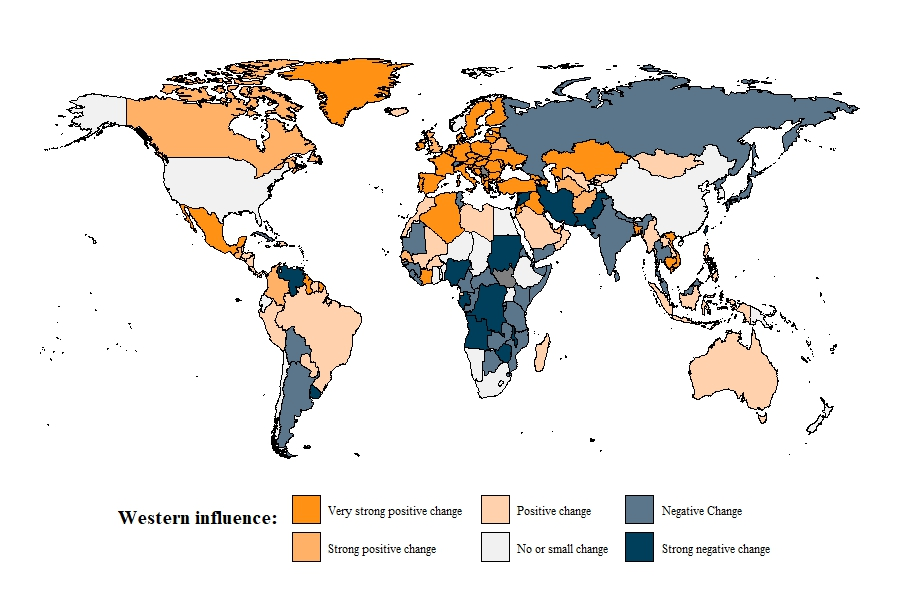
\includegraphics[width = \textwidth]{western_influence.jpeg}
\caption{Change in Western influence}
\label{fig:west}
\end{figure}

Now, displacement is just a speculation on my side, and we need some proof that this is happening. Figure \ref{fig:west} shows changes in Western\footnote{I have defined the west in this case as any country belonging to the 27 EU countries, as well as all countries with a strong democratic history since at least the 1990s. The actual countries included in the definition of `The West' can be found in Appendix \ref{apn:notes}.} influence for all countries. The orange colour indicates a positive change in linkages to the West, while the blue colour indicates a negative change. Comparing Figures \ref{fig:link-china} and \ref{fig:west}, we can see that there are some noticeable traces of displacement happening, especially in sub-Saharan Africa. The opposite is true for Europe, where European integration is likely to have caused Western linkages to strengthen. However, there seems to be a trend of China displacing Western linkages in some regions of the world, especially sub-Saharan Africa and Central Asia. It would not be unreasonable to think that the change in East-Asia should be far more negative, but the likely reason as to why the West is maintaining its position in Southeast Asia, is because my definition of the West includes Japan, South Korea, and Taiwan, which are major economic partners to the Southeast Asian countries. 

It is likely that much of the displacement is caused by China's rise as an economic powerhouse. China is the world's second largest economy, and one of the only great economies that are not Western and democratic. The economic power of China increases China's own heft and norms in the region it displaces Western countries, while at the same time decreasing the power Western countries has to oppose restrictions on freedom of expression. 

Another way in which China can possibly displace the West is in the realm of security. China is the world's fourth largest arms provider \citep{george_trends_2025, gunter_chinas_2024}, comprising almost six per cent of global exports between 2020 and 2024. However, this is lower than the previous period measured by SIPRI \citep{george_trends_2025}. This decline might be down to the fact that China has been rebuilding its military for several years, devoting more of its production to domestic use. The focus on domestic use could perhaps strengthen China as a security partner, a role they are seeking to expand. At the same time, However, China is actively seeking to avoid being entangled in other countries' conflicts, so the only real military alliance China has is with North Korea. Showcasing the country's ambivalence to becoming a security guarantor. This makes it doubtful that security linkages are of consequence for displacement, but the fact that China's arms manufacturers have fewer restrictions on whom they sell to \citep{gunter_chinas_2024}, might serve to displace Western influence in some areas.

To some extent, China is also seeking to displace the West in the realm of diplomacy. China has become an important diplomatic partner to many countries, and its position on the UN Security Council makes it very powerful. China has ambitions of creating a more China-centric sphere of influence, sometimes termed the China Model or Beijing Consensus\footnote{The latter as a play on the famous Washington Consensus.} \citep{ambrosio_rise_2012, economy_exporting_2020}. This is perhaps most clear in the Shanghai Cooperation Organisation (SCO), which is an international organisation made up of ostensibly authoritarian Central Asian countries, with by far the most powerful country being China. The organisation is a conservative one, established to preserve autocratic regimes in the region \citep[p. 1322]{ambrosio_catching_2008}.

As linkages to the West gets replaced with linkages to China, the power Western countries have to sanction restrictions on freedom of expression becomes smaller. This can be used by willing domestic elites to repress freedom of expression, who are safe knowing that China will back them up.

\section{Expectations} \label{sec:hypotheses}
The third wave of autocratisation offers us many cases to study, each of which will be slightly different from all the others. But one of the major changes that has occurred in conjunction with this wave is the rise of China. This is an interesting coincidence, and we should ask the question: are these two phenomena in any way connected?

Previous literature on the subject indicates that we should not expect a concerted effort from China's side to push autocratisation or put pressure on freedom of expression. Although this is certainly possible in some cases of particular interest to China, such as Hong Kong \citep{chen_democracy_2015}. We should rather expect to see a gradual change occurring through repeated interactions with China. Through learning, immunity, and displacement, linkages to China offers domestic elites who are inclined to limit freedom of expression a way to do this that negates consequences like economic sanctions. It might also give aspiring autocratisers in democracy the know-how to restrict freedom of expression by giving access to technologies through trade and strategies through diplomatic and social channels. 

When China has established the linkages, they begin to have a gradual effect on the partner country's level of freedom of expression. I theorise that there are three main mechanisms through which this effect is channelled: learning, immunity, and displacement. The confluence of these factors leads us to hypothesis one:
\begin{displayquote}
    \textit{H\textsubscript{1}: An increase in linkages to China will have a negative effect on the level of freedom of expression.}  
\end{displayquote}

From previous research \citep{toettoe_foreign_2023}, we know that hybrid regimes are more likely to be affected than other types of regimes. Hybrid, sometimes known as transitory, regimes are the regimes that displays both democratic and authoritarian characteristics. This gives rise to a secondary hypothesis where hybrid regimes are more likely to be affected by linkages than are institutionalised ones. Where electoral autocracies and democracies are likely to be swayed by international pressure, this is less likely to affect closed autocracies and liberal democracies. I reason that this is because the level of freedom of expression is rather set, or institutionalised, in these societies. They will usually have robust institutions that either defend against attacks on freedom of expression, in the case of liberal democracies, or have institutions that restrict repress freedom of expression, in the case of closed autocracies. This institutionalisation is likely the exception in hybrid regimes. Hybrid regimes thread a fine line between democracy and autocracy; their regimes usually having a combination of `virtuous' and `perverse' institutions, where democratic and authoritarian characteristics are blended together \citep{valenzuela_democratic_1990}. Hybrid regimes are also more likely to change scores on freedom of expression, because many can be, but are not necessarily, in a transitory phase; either democratising or autocratising.

I expect there to be a ceiling and floor effect at play, which must be accounted for. On the one hand, liberal democracies cannot increase their level of freedom of expression, because it is almost at the very limit of how unrestricted it can be. On the other hand, we find the closed autocracies, where freedom of expression is so low that it cannot reasonably be degraded any further. This leads to secondary hypothesis:
\begin{displayquote}
    \textit{H\textsubscript{2}: An increase in linkages to China will have a stronger negative effect on freedom of expression in hybrid regimes.}
\end{displayquote}

These are the two hypotheses I set out to study in the next chapters. The rest of the thesis I dedicate to creating a method of studying these expectations, analysing the results, and discussing what I find. 